\documentclass[10pt,pscyr,nonums]{hedlab}
\usepackage[russian]{babel}
\usepackage{hedmaths}
\usepackage{graphicx}
\graphicspath{{plots/}, {images/}}

\newgeometry{top=1.5cm, bottom=1.5cm, left=1cm, right=1cm}

\student{} \date{}
\labnum{5}
\labname{Определение параметров тиратрона}
\begin{document}
    \makeheader

    \emph{Цель работы:} знакомство с управляемыми газоразрядными приборами,
    построение вольтамперной и пусковой характеристик тиратрона.
    
    \begin{figure}[h!]
        \center
        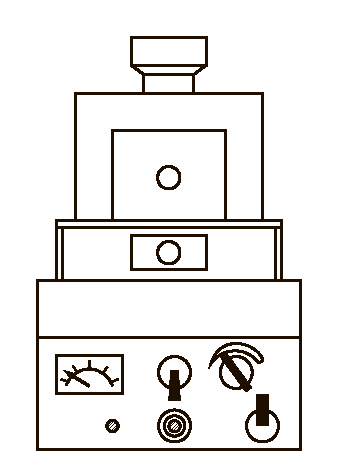
\includegraphics[width=.37\textwidth]{appearance} \hspace*{2em}
        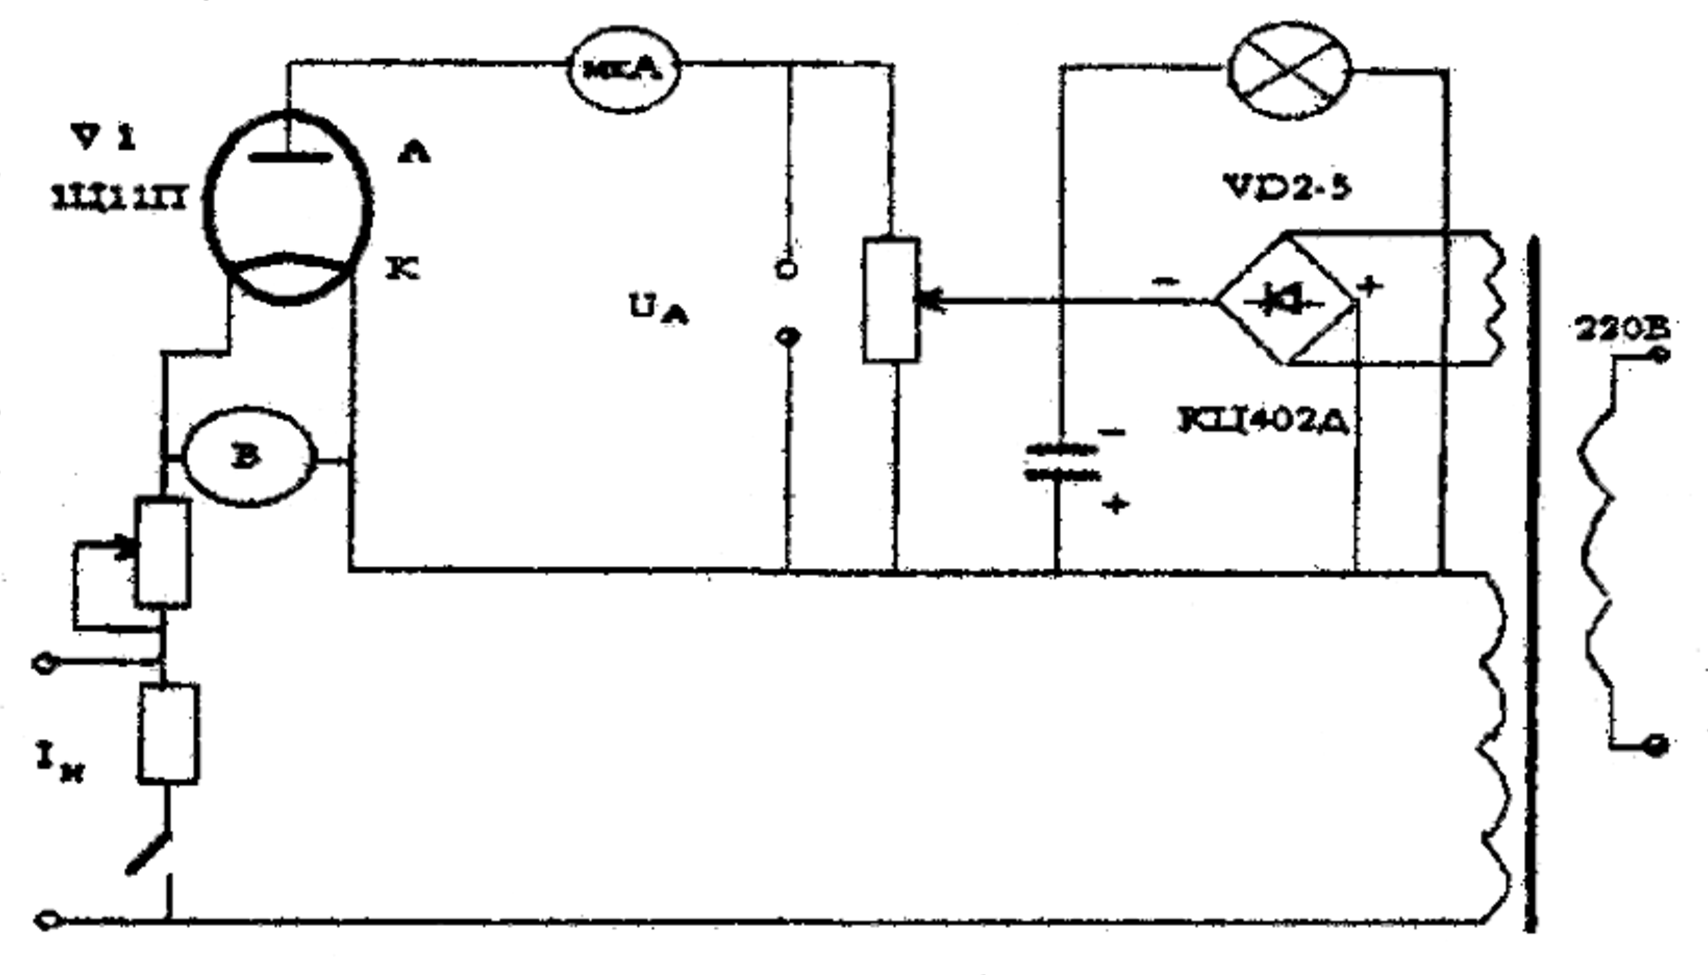
\includegraphics[width=.45\textwidth]{scheme}
        \parbox{.37\textwidth}{\caption{Лабораторная установка}}
        \hspace*{2em}
        \parbox{.45\textwidth}{\caption{Принципиальная схема установки}}
    \end{figure}
    
    \vspace*{2em}
    
    \begin{table}[h!]
        \center
        \caption{Пусковая характеристика тиратрона}
        \begin{tabular}{|m{.1\textwidth}|*{8}{m{.06\textwidth}|}} \hline
            \( U_c \), В &&&&&&& \\ \hline
            \( U_A \), В &&&&&&& \\ \hline
            \( U_A \), В &&&&&&& \\ \hline
            \( U_A \), В &&&&&&& \\ \hline
            \( \midnum{U_A} \), В &&&&&&& \\ \hline
        \end{tabular}
    \end{table}
    
    \pagebreak
    
    \begin{table}[h!]
        \center
        \caption{Зависимость анодного тока от напряжения}
        \begin{tabular}{|m{.1\textwidth}|*{10}{m{.06\textwidth}|}} \hline
            \multicolumn{11}{|c|}{\( U_{c_1} = \)} \\ \hline
            \( U_A \), В &&&&&&&&&& \\ \hline
            \( I_A \), В &&&&&&&&&& \\ \hline
            \multicolumn{11}{|c|}{\( U_{c_2} = \)} \\ \hline
            \( U_A \), В &&&&&&&&&& \\ \hline
            \( I_A \), В &&&&&&&&&& \\ \hline
            \multicolumn{11}{|c|}{\( U_{c_3} = \)} \\ \hline
            \( U_A \), В &&&&&&&&&& \\ \hline
            \( I_A \), В &&&&&&&&&& \\ \hline
            \multicolumn{11}{|c|}{\( U_{c_4} = \)} \\ \hline
            \( U_A \), В &&&&&&&&&& \\ \hline
            \( I_A \), В &&&&&&&&&& \\ \hline
            \multicolumn{11}{|c|}{\( U_{c_5} = \)} \\ \hline
            \( U_A \), В &&&&&&&&&& \\ \hline
            \( I_A \), В &&&&&&&&&& \\ \hline
            \multicolumn{11}{|c|}{\( U_{c_6} = \)} \\ \hline
            \( U_A \), В &&&&&&&&&& \\ \hline
            \( I_A \), В &&&&&&&&&& \\ \hline
            \multicolumn{11}{|c|}{\( U_{c_7} = \)} \\ \hline
            \( U_A \), В &&&&&&&&&& \\ \hline
            \( I_A \), В &&&&&&&&&& \\ \hline
            \multicolumn{11}{|c|}{\( U_{c_8} = \)} \\ \hline
            \( U_A \), В &&&&&&&&&& \\ \hline
            \( I_A \), В &&&&&&&&&& \\ \hline
        \end{tabular}
    \end{table}   
\end{document}
